\documentclass[french, 12pt]{article}
\usepackage[a4paper, top=2cm, bottom=2cm, left=2cm, right=2cm]{geometry}

\usepackage[mono=false]{libertine}
\usepackage[french]{babel}
\usepackage{hyperref}
\usepackage{microtype}
\usepackage{textcomp}
\usepackage[bottom]{footmisc}
\usepackage{graphicx}
\usepackage{siunitx}
\usepackage{multirow}
\usepackage{makecell}
\usepackage{booktabs}

\DeclareSIUnit\octet{o}

\sisetup{
    detect-all,
    output-decimal-marker={,},
    group-minimum-digits = 3,
    group-separator={~},
    number-unit-separator={~}
}

\newcommand{\rpi}{\emph{Raspberry Pi}}


\title{Pi-kachULM\_OS}
\author{}
% \author{Émile Sauvat, Hubert Gruniaux \& Gabriel Desfrene}  % Mettre en bas de page.
\date{}

\begin{document}
\maketitle

\section{Présentation}
\subsection{Objectif}
Nous nous sommes fixés comme objectif premier la réalisation d'un système
d'exploitation en C++ s'exécutant sur une
\href{https://www.raspberrypi.com/products/raspberry-pi-3-model-b-plus/}{\emph{Raspberry Pi 3B+}}.
Ce choix était principalement motivé par le support de cette plateforme par
l'émulateur \href{https://www.qemu.org/}{\emph{QEMU}}.

Finalement, par curiosité et pour le fun\texttrademark, nous avons finalement
choisi de supporter plusieurs modèle de \rpi{} :
\begin{itemize}
    \item \href{https://www.raspberrypi.com/products/raspberry-pi-3-model-b-plus/}{\emph{Raspberry Pi 3B+}}
    \item \href{https://www.raspberrypi.com/products/raspberry-pi-4-model-b/}{\emph{Raspberry Pi 4 Model B}}
    \item \href{https://www.raspberrypi.com/products/compute-module-4/?variant=raspberry-pi-cm4001000}{\emph{Raspberry Pi Compute Module 4}}
\end{itemize}

La totalité de ce qu'il suit à donc été testé et conçu afin d'être exécuté sur
l'un de ces modèles. Ce projet compte environ \num{10000} lignes de codes de
C++, \num{700} lignes de C et \num{150} lignes d'assembleur ARM64. La totalité du code
est disponible à l'adresse suivante : \url{https://github.com/hgruniaux/Pi-kachULM_OS}


% $ cloc -vcs=git kernel/ lib/ tools/ binuser/
%      178 text files.
%      177 unique files.
%       13 files ignored.

% github.com/AlDanial/cloc v 1.98  T=0.06 s (2986.6 files/s, 278145.5 lines/s)
% -------------------------------------------------------------------------------
% Language                     files          blank        comment           code
% -------------------------------------------------------------------------------
% C++                             64           1900            809           6759
% C/C++ Header                    82            994            975           3374
% C                               17            171             18            691
% CMake                            8             80             21            253
% Assembly                         2             40             50            150
% Bourne Shell                     2             27              8             81
% Linker Script                    1              9              6             39
% Markdown                         1             10              0             19
% -------------------------------------------------------------------------------
% SUM:                           177           3231           1887          11366
% -------------------------------------------------------------------------------

% With deleted files:
% On branch update-cmake
% Changes not staged for commit:
%   (use "git add/rm <file>..." to update what will be committed)
%   (use "git restore <file>..." to discard changes in working directory)
%         deleted:    binuser/stb_image.c
%         deleted:    binuser/stb_image.h
%         deleted:    kernel/fs/fat/diskio.h
%         deleted:    kernel/fs/fat/ff.c
%         deleted:    kernel/fs/fat/ff.h
%         deleted:    kernel/fs/fat/ffconf.h
%         deleted:    kernel/fs/fat/ffunicode.c
%         deleted:    kernel/graphics/stb_image.c
%         deleted:    kernel/graphics/stb_image.h
%         deleted:    kernel/wm/data/pika_icon.cpp
%         deleted:    kernel/wm/data/pika_icon.hpp
%         deleted:    lib/libk/src/format.cpp
%
% no changes added to commit (use "git add" and/or "git commit -a")

\subsection{Reconnaissance dynamique du matériel}
Afin de supporter plusieurs machines, qui ne partagent pas toutes les mêmes
caractéristiques et spécificités nous avons besoin d'un moyen de les déterminer
dynamiquement, lors du démarrage du noyau. Pour ce faire, le noyau utilise et le
\textit{DeviceTree} donné par le \textit{bootloader}. Nous avons donc développé
une bibliothèque, \mbox{\texttt{libdevice-tree}} permettant d'interpreter cette
structure.

Un \textit{DeviceTree} est, comme son nom l'indique, un arbre, compilé sous la
forme d'un fichier binaire, qui est chargé par le \textit{bootloader} lors du
démarrage. Cet arbre est rempli par ce dernier, et informe le noyau du matériel
présent. Une documentation est disponible sur cette
\href{https://www.devicetree.org/specifications/}{page}.

\section{Modèle mémoire}
\subsection{Vue de la mémoire}
Lors du démarrage du système d'exploitation, ce dernier récupère la taille de la
mémoire disponible et s'occupe d'initialiser le \textit{Memory Management Unit (MMU)}
pour que le noyau puisse s'abstraire de la mémoire physique. Cette configuration
est effectuée au sein du fichier \texttt{mmu\_init.cpp}. Les pages ont une
taille fixée à $\SI{4}{\kibi\octet}$.

On utilise ici à bon escient les spécificités du \textit{MMU} de la plateforme
ARM. Cette dernière nous permet d'avoir deux espaces d'adressage complètement
distincts :

\begin{itemize}
    \item La mémoire des processus est dans l'espace d'adresse \texttt{0x0000000000000000} à \texttt{0x0000ffffffffffff}.
    \item La mémoire du noyau est, elle, dans l'espace d'adresse \texttt{0xffff000000000000} à \texttt{0xffffffffffffffff}.
          La table \ref{tbl:memory-mapping} décrit l'origanisation de cette
          plage d'adresse au sein de notre noyau.
\end{itemize}

\begin{table}[ht]
    \begin{center}
        \begin{tabular}{|c|c}
            \cline{1-1}
            \multirowcell{3}{1:1 \textit{mapping}                               \\ \scriptsize Code du noyau, \textit{Device Tree}}
                                            & \texttt{0xffff\,0000\,0000\,0000} \\ \\ \\
            \cline{1-1}
            \multirowcell{3}{Mémoire Vidéo} & \texttt{0xffff\,1000\,0000\,0000} \\ \\ \\
            \cline{1-1}
            \multirowcell{3}{Mémoire périphériques                              \\ \scriptsize \textit{MMIO}}
                                            & \texttt{0xffff\,2000\,0000\,0000} \\ \\ \\
            \cline{1-1}
            \multirowcell{3}{Pages Utilisateurs                                 \\ \scriptsize programme, tas et pile des programmes utilisateurs}
                                            & \texttt{0xffff\,3000\,0000\,0000} \\ \\ \\
            \cline{1-1}
            \multirowcell{3}{\textit{Buffers} DMA}
                                            & \texttt{0xffff\,4000\,0000\,0000} \\ \\ \\
            \cline{1-1}
            \multirowcell{3}{Tas du Noyau                                       \\ \scriptsize grandissant vers le bas}
                                            & \texttt{0xffff\,5000\,0000\,0000} \\ \\ \\
            \cline{1-1}
            \multirowcell{3}{Système de Fichier en RAM}
                                            & \texttt{0xffff\,a000\,0000\,0000} \\ \\ \\
            \cline{1-1}
            \multirowcell{3}{Pile du Noyau                                      \\ \scriptsize grandissant vers le haut}
                                            & \texttt{0xffff\,f000\,0000\,0000} \\ \\
                                            & \texttt{0xffff\,ffff\,ffff\,ffff} \\
            \cline{1-1}
        \end{tabular}
    \end{center}
    \caption{Vue de la mémoire au sein de l'espace noyau.}
    \label{tbl:memory-mapping}

\end{table}
% Do a scheme of the memory mapping

\subsection{Allocateurs de pages}
Une fois que le noyau est passé en mémoire virtuelle, il nous faut un moyen
de garder une trace des pages physiques libres ou utilisées par le noyau. Pour
ce faire, nous avons implémenté deux allocateur de pages :
\begin{itemize}
    \item \texttt{page\_alloc.hpp} s'occupe de l'allocation de la grande
          majorité des pages physiques de la mémoire. Cette allocation est
          réalisée de manière optimisée par un arbre binaire. 

          Chaque nœud est composé d'un bit de donné indiquant si au moins une
          page (=une feuille) est libre parmis tout ses descendant, ou si la page 
          est libre s'il s'agit d'une feuille. Ainsi on peut accéder à la disponibilité
          de chaque page en temps constant. On peut également trouver une page disponible, 
          sous réserve d'existence, en $\bigcirc (\log n)$ temps, étant donné qu'on élimine 
          la moitié des page existantes à chaque étape de descente dans l'arbre, 
          le tout en gardant constament une page libre au moins parmis les descendants 
          envisagés. 
          
          La libération d'une page doit se faire en modifiant les ancêtre 
          nécessaires pour prendre en compte la disponibilité de la page, donc en au plus 
          $\bigcirc (\log n)$ temps également. 

    \item \texttt{contiguous\_page\_alloc.hpp} travaille sur une petite portion
          de la mémoire physique ($\approx \SI{100}{\mebi\octet}$) et s'occupe
          d'allouer une liste de pages contiguës. Cette allocation est
          nécessaire pour la création des \textit{buffers} utilisés lors des
          transferts DMA.
\end{itemize}

\subsection{Allocateurs de mémoire}
À l'aide de l'allocateur de page principal et en modifiant les tables de
translation du \textit{MMU} du noyau, un \textit{heap} est simulé à partir des
adresses \texttt{0xffff500000000000}.
En utilisant une structure de liste doublement chainée de \textit{MetaBlock}, on alloue la mémoire requise 
linéairement dans le heap, ainsi que les données suivantes :
\begin{itemize}
    \item La taille \textit{size} du bloc mémoire, sans compter le décalage permettant l'alignement 
    du début du block si celui-ci est alloué.
    \item Les block suiants et précédent \textit{next} et \textit{previous}
    \item L'adresse de début de la mémoire allouée, sous la forme d'un pointeur et d'une adresse vers un tableau 
    de charactères.
\end{itemize}

Ces block permettent de manipuler plus facilement les blocks mémoire, notamment pour les séparer en deux si le 
block alloué est trop grand ou pour fusionner deux block libres consécutifs.

\subsection{Système de fichier}
Nous utilisons les \textit{bootloader} des \rpi{} afin de charger une
image disque en mémoire à l'adresse physique \texttt{0x0x18000000}. Après
configuration du \textit{MMU}, nous sommes en mesure d'accéder à cette image
depuis l'adresse virtuelle \texttt{0xffffa00000000000}.

Cette image disque est celle d'une partition FAT contenant les programmes
utilisées et disponible dans notre système d'exploitation. La bibliothèque
permettant de lire cette partition n'a pas été développé par nos soins, elle est
disponible à l'adresse suivante : \url{http://elm-chan.org/fsw/ff/}. Les
quelques fonctions nécessaire à son bon fonctionnement sont trouvables dans le
fichier \texttt{ramdisk.cpp}.

\section{\textit{Drivers}}
Plusieurs \textit{drivers} ont été développé au cours de ce projet afin
d'interagir avec les différents périphériques présent sur les \rpi{} supportés.
Ils ont tous été développé à l'aide des documentations fournies par \rpi{}:
\begin{itemize}
    \item \emph{Raspberry Pi 3B+} : \url{https://datasheets.raspberrypi.com/bcm2835/bcm2835-peripherals.pdf}
    \item \emph{Raspberry Pi 4} : \url{https://datasheets.raspberrypi.com/bcm2711/bcm2711-peripherals.pdf}
\end{itemize}

\subsection{GPIO}
Le premier pilote développé est celui qui est essentiel pour la communication
à l'extérieur. Ce pilote s'occupe d'initialiser et de contrôler les 40
\textit{pins} disponibles sur les \rpi{}. La figure \ref{img:gpio} donne les
fonctions de ces 40 connecteurs. Le pilote développé au sein du fichier
\texttt{gpio.cpp} permet de lire et fixer les niveaux logiques, de configurer
les résistances de \textit{pull-up} ainsi que de traiter les interruptions
générées par les changements de de niveau.

\begin{figure}[htp]
    \begin{center}
        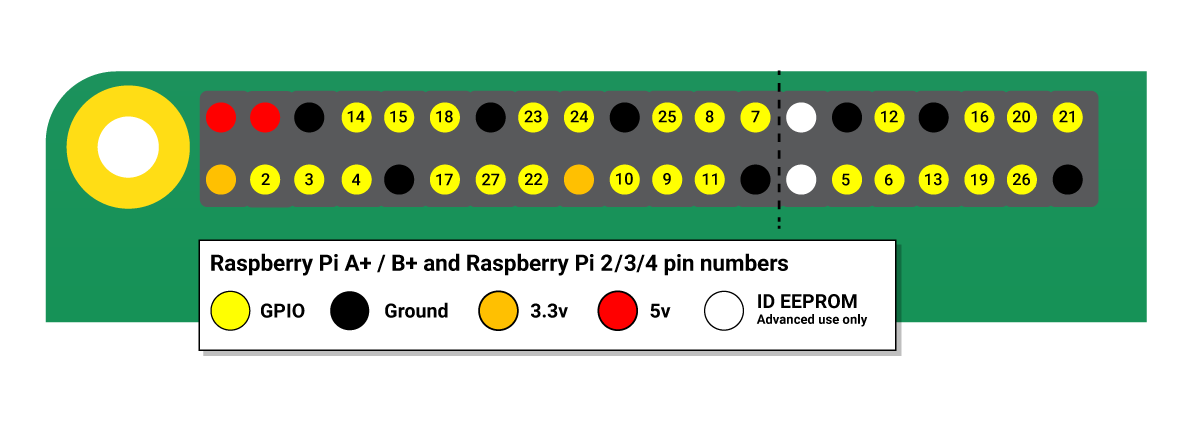
\includegraphics[height=5cm]{gpio.png}
    \end{center}
    \caption{Les 40 \textit{pins} disponibles sur les \rpi{}.}
    \label{img:gpio}
\end{figure}

\subsection{Mini UART}
Un pilote afin d'utiliser l'implementation d'UART par \emph{Broadcom},
Mini UART, a été développé au sein du fichier \texttt{miniuart.cpp}. Celui-ci
permet d'établir une communication \emph{serial}. Bien que fonctionnel, nous
l'avons utilisé afin de fixer les problèmes du notre pilote UART, plus fiable.
En effet, l'horloge de Mini UART est celle du GPU présent, ce qui limite la
vitesse en baud de communication (et la rend impossible lors du changement
d'horloge du GPU !).

\subsection{UART}
Un pilote UART qui est essentiel pour le débogage est présent au sein du noyau
(dans le fichier \texttt{uart.cpp}). Celui-ci permet d'interagir avec les
\href{https://developer.arm.com/Processors/PL011}{PL011} présent sur les cartes.
La communication \textit{serial} se fait, comme pour Mini UART, via les
\textit{pins} 14 et 15 du GPIO. Nous avons utilisé le
\textit{Raspberry Pi Debug Probe}, en figure \ref{img:debug-probe}, afin
d'établir une communication \textit{serial} entre les \rpi{} et nos ordinateurs.

\begin{figure}[htp]
    \begin{center}
        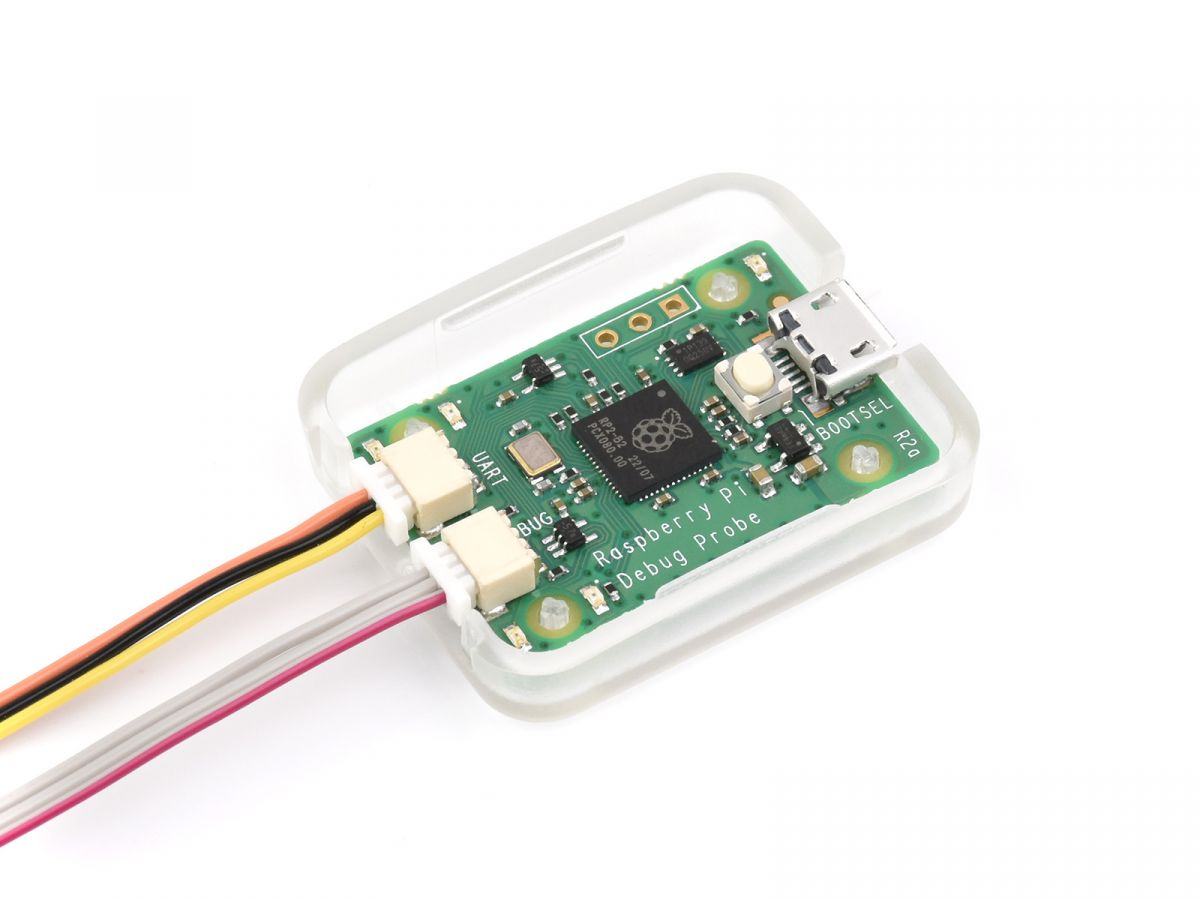
\includegraphics[height=5cm]{debug-probe.jpg}
    \end{center}
    \caption{Le \textit{Raspberry Pi Debug Probe}, l'adaptateur \textit{serial}
        vers \textit{USB} que nous avons utilisé.}
    \label{img:debug-probe}
\end{figure}


\subsection{\textit{Mailbox} du \textit{VideoCore}}
La \textit{Mailbox} du \textit{VideoCore}%
\footnote{Nom des GPU présent sur les \rpi{} développé par \emph{Broadcom}.}
permet d'interagir facilement avec certains périphériques présent sur le
SoC. Elle permet par exemple l'allocation des \textit{Framebuffer}
pour la video, la configuration des horologes ou le contrôle des LED d'activité.
Un pilote permettant de communiquer via le protocole \textit{Mailbox} au GPU est
donc présent donc notre noyau, au sein du fichier \texttt{mailbox.cpp}.

\subsection{Contrôleurs IRQ}
Afin de gérer les interruptions générées par les périphériques, nous avons du
développer des contrôleurs IRQ. Cependant, les deux SoC sur lesquels nous avons
travaillés le BCM2711 et le BCM2835 ne possèdent pas les mêmes contrôleurs IRQ.
Deux pilotes ont donc été intégrés au noyau, l'un propre au BCM2711, l'autre
pour le \href{https://developer.arm.com/Processors/CoreLink%20GIC-400}{GIC-400},
présent sur les \textit{Raspberry Pi 4}. Ces pilotes sont disponibles au sein du
dossier \texttt{kernel/hardware/irq}.

\subsection{Contrôleur DMA}
Un pilote DMA a été développé afin de procéder à des copies entres des segments
de la mémoire. Sur les \rpi{}, ce contrôleur est directement relié au bus
utilisés par tous les périphériques pour communiquer, ce qui permet d'interagir
directement avec eux. Ce pilote supporte par exemple, la copie de l'horloge du
système directement vers l'UART, sans passer par le CPU. La connection du
contrôleur directement au bus implique cependant que toutes les copies
interagissant sur la SDRAM doivent être linéairement selon les adresses
physiques. Cela a motivé le développement des \textit{Buffer} DMA.

Ce pilote semble fonctionnel, cependant des problèmes sont apparu lors de
l'utilisation du DMA pour de copier les fenêtres des processus sur le
\textit{framebuffer}. Plus de tests sont nécessaire pour s'assurer de son bon
fonctionnement.

\subsection{Horloge Système}
Un pilote pour l'horloge du système, partagée entre les cœurs du CPU est présent
au sein du noyau. Celui-ci permet de configurer le lancement d'IRQ de manière
récurrente ou non. Le pilote est trouvable au sein du fichier
\texttt{system\_hardware.cpp}.

\subsection{Timer ARM}
Un pilote pour l'horloge de chaque cœur ARM est également au sein du noyau.
Cependant, celui-ci ne supporte pas la configuration du lancement d'IRQ. Il
reste très utile afin de récupérer à faible coût le temps écoulé depuis le
démarrage du noyau.

\section{Processus}

Une implémentation de processus et threads est proposé dans notre OS. Celle-ci bien que imparfaite, propose tout de même de multiples fonctionnalités et reste flexible pour de futurs améliorations. Elle est lourdement inspiré de l'implémentation de Linux.

\subsection{Hiérarchie}

Au niveau de notre noyau, la notion de processus n'existe pas, ni celle de thread. Tout est une tâche (représentée par la classe C++ \texttt{Task}). Une tâche est de façon générale une opération qui peut être préempté ou ordonnancé : cela désigne donc tout objet qui sera manipulé par le scheduler.

Une tâche a systématiquement son propre stack et peut avoir optionnellement sa propre mémoire virtuelle. Il peut tourner à la fois en espace utilisateur (niveau EL0) ou en espace noyau avec un stack distinct (niveau EL1). Chaque tâche maintient aussi sa propre liste de fenêtre (pour le window manager) et de fichier ouverts.

Un processus est alors simplement une tâche qui tourne en espace utilisateur avec sa propre mémoire virtuelle. Un thread est une tâche qui partage les mêmes fichiers/fenêtres et la même mémoire virtuelle qu'avec une autre tâche (qui joue le rôle de processus parent).

\subsection{Appels systèmes}

Afin qu'une tâche puisse communiquer avec le noyau, un ensemble d'appels systèmes est supporté. Ces derniers se font avec la même convention que Linux: les arguments sont passés dans les registres \texttt{r0} à \texttt{r7}, l'identifiant de l'appel est passé dans \texttt{w8} et l'appel lui-même est effectué par l'instruction \texttt{svc \#0}.

L'interprétation de l'identifiant et des arguments est fait par la table des syscalls. Cette dernière est spécifique à chaque tâche (aussi bien noyau qu'espace utilisateur). Toutefois, une seule table des syscalls a été implémenté dans notre noyau pour le moment. Elle est donnée dans \ref{syscall_table}.

Tous les syscalls ne peuvent pas forcèment être appelé par des tâches noyaux.

\begin{table}[]
\label{syscall_table}
\centering
\begin{tabular}{@{}ll@{}}
\toprule
Fonction C  & Description \\ \midrule
\texttt{sys\_exit}   & Tue la tâche avec un le code erreur donnée \\
\texttt{sys\_print}  & Affiche du texte dans le log noyau \\
\texttt{sys\_getpid}  & Renvoie l'identifiant de la tâche \\
\texttt{sys\_debug}  & Affiche un entier dans le log noyau \\
\texttt{sys\_spawn}  & Creé un nouveau processus enfant à partir du fichier ELF donnée \\
\texttt{sys\_sleep}  & Mets en pause la tâche pour le temps donné au minimum \\
\texttt{sys\_yield}  & Passes le contrôle à d'autres tâches \\
\texttt{sys\_sched\_get\_priority}  & Recupère la priorité actuelle de la tâche \\
\texttt{sys\_schet\_set\_priority}  & Définit la nouvelle priorité de la tâche \\
\texttt{sys\_sbrk}  & Change la position du heap (allocation de mémoire) \\
\texttt{sys\_open\_file} & Ouvre un fichier \\
\texttt{sys\_close\_file} & Ferme un fichier \\
\texttt{sys\_read\_file} & Lit des octects à partir d'un fichier ouvert \\
\texttt{sys\_get\_file\_size} & Renvoie la taille d'un fichier ouvert \\
\texttt{sys\_open\_dir} & Ouvre un répertoire \\
\texttt{sys\_close\_dir} & Ferme un répertoire \\
\texttt{sys\_read\_dir} & Lit une entrée du répertoire \\
\texttt{sys\_poll\_message} & Récupère un message d'une fenêtre si disponible \\
\texttt{sys\_wait\_message} & Comme \texttt{sys\_poll\_message} mais bloque si plus de message \\
\texttt{sys\_window\_create} & Crée une fenêtre \\
\texttt{sys\_window\_destroy} & Détruit une fenêtre \\
\texttt{sys\_window\_set\_title} & Mets à jour le titre d'une fenêtre \\
\texttt{sys\_window\_get\_visibility} & Récupère la visibilité actuelle d'une fenêtre \\
\texttt{sys\_window\_set\_visibility} & Affiche ou cache une fenêtre \\
\texttt{sys\_window\_get\_geometry} & Récupéré la position et la taille d'une fenêtre \\
\texttt{sys\_window\_set\_geometry} & Déplace ou redimensionne une fenêtre \\
\texttt{sys\_window\_present} & Redessine la fenêtre à l'écran \\
\texttt{sys\_gfx\_clear} & Efface le contenu d'une fenêtre par une couleur \\
\texttt{sys\_gfx\_draw\_line} & Affiche une ligne dans une fenêtre \\
\texttt{sys\_gfx\_draw\_rect} & Affiche un rectangle dans une fenêtre \\
\texttt{sys\_gfx\_fill\_rect} & Remplit un rectangle dans une fenêtre \\
\texttt{sys\_gfx\_draw\_text} & Affiche du texte dans une fenêtre  \\
\texttt{sys\_gfx\_blit} & Copie une image 2D dans une fenêtre \\ \bottomrule
\end{tabular}
\caption{Table des syscalls}
\end{table}

\section{Ordonnanceur}
\subsection{Algorithme et Priorités}

Le noyau utilise un scheduler préemptif pour déterminer la prochaine tâche à exécuter. Son algorithme exact est donné ici.

Toutes les tâches qui peuvent être actuellement exécutées sont réparties dans 32 queues en fonction de leur priorité. À chaque tick de l'horloge, s'il y a une tâche dans une queue de priorité plus élevée que la tâche actuelle, alors cette tâche est choisie pour être exécutée (même si le budget de temps n'est pas encore dépassé). Autrement, si le budget de temps de la tâche actuelle est dépassé (10 ms par défaut, dépend de la priorité de la tâche), alors la prochaine tâche est choisie dans la queue de priorité actuelle ou plus basse. La tâche précédente étant à nouveau ajoutée à la fin de la queue correspondant à sa priorité (algorithme round-robinn).

\subsection{Mise en pause de Processus}

Lorsqu'une tâche est mise en pause, on la retire des queues du scheduler. Pour la réveiller, il suffit de l'insérer un nouveau dans la queue correspondant à sa priorité.

Dans le cas d'un endormissement pour une certaine durée, la tâche est mise dans une delta queue. Dans cette structure de donnée, on préserve seulement le temps restant (avant le réveil) \textbf{relativement} à la tâche précédente dans la delta queue. De cette façon, la mise à jour de la queue est faite en temps constant (il suffit de mettre à jour la tête de la queue). Une fois le temps écoulé, on replace la tâche dans une des queues d'exécution du scheduler.

\section{Écran et Fenêtres}
\subsection{\textit{Framebuffer}}

Au démarrage du noyau, une requête mailbox est effectuée pour allouer un framebuffer pour l'écran auprès du VideoCore (carte graphique intégrée de la Raspberry PI). Ce framebuffer n'est jamais réalloué plus tard et est directement modifié pour mettre à jour l'écran.

Normalement, un mécanisme de détection de la taille de l'écran est en place, mais ne marche pas en pratique (renvoie des tailles d'écran qui ne correspondant pas à la résolution native). De plus, un système de double buffering est aussi implémenté en utilisant les virtuals offsets du VideoCore, mais il ne fonctionne pas non plus sur le hardware.

\subsection{Gestionnaire de fenêtres}

Chaque tâche a la possibilité de créer une ou plusieurs fenêtres. Pour chaque fenêtre, un framebuffer est alloué en espace noyau pour stocker son contenu et une queue des messages est créé. La tâche utilisateur peut alors dessiner dans le framebuffer via des syscalls ou recevoir des messages du noyau sur les faits et gestes de la fenêtre (entrés claviers, déplacement, redimensionnement, fermeture demandée, etc.).

Le window manager en lui-même est une tâche noyau qui vérifie régulièrement s'il y a eu des modifications (déplacement de fenêtre, changement de focus, fenêtre mise à jour, etc.) et compose les fenêtres à l'écran. C'est également ce dernier qui est responsable de dessiner l'arrière-plan (une image chargée à partir du système de fichier).  Les décorations d'une fenêtre sont dessinées par le window manager dans le framebuffer de la fenêtre juste avant le blit vers le framebuffer global de l'écran.

\section{Clavier PS/2}
Afin d'interagir facilement avec l'interface de notre noyau, nous avons
développé une interface ainsi qu'un pilote afin d'utiliser un clavier PS/2 sur
les \rpi{}. Le protocole PS/2 n'étant pas supporté nativement par ces
ordinateurs nous avons du construire un petit circuit électronique, visible en
figure \ref{img:ps2-cables}, afin de connecter un clavier aux \textit{pins} du
\textit{GPIO}.

\begin{figure}[htp]
    \begin{center}
        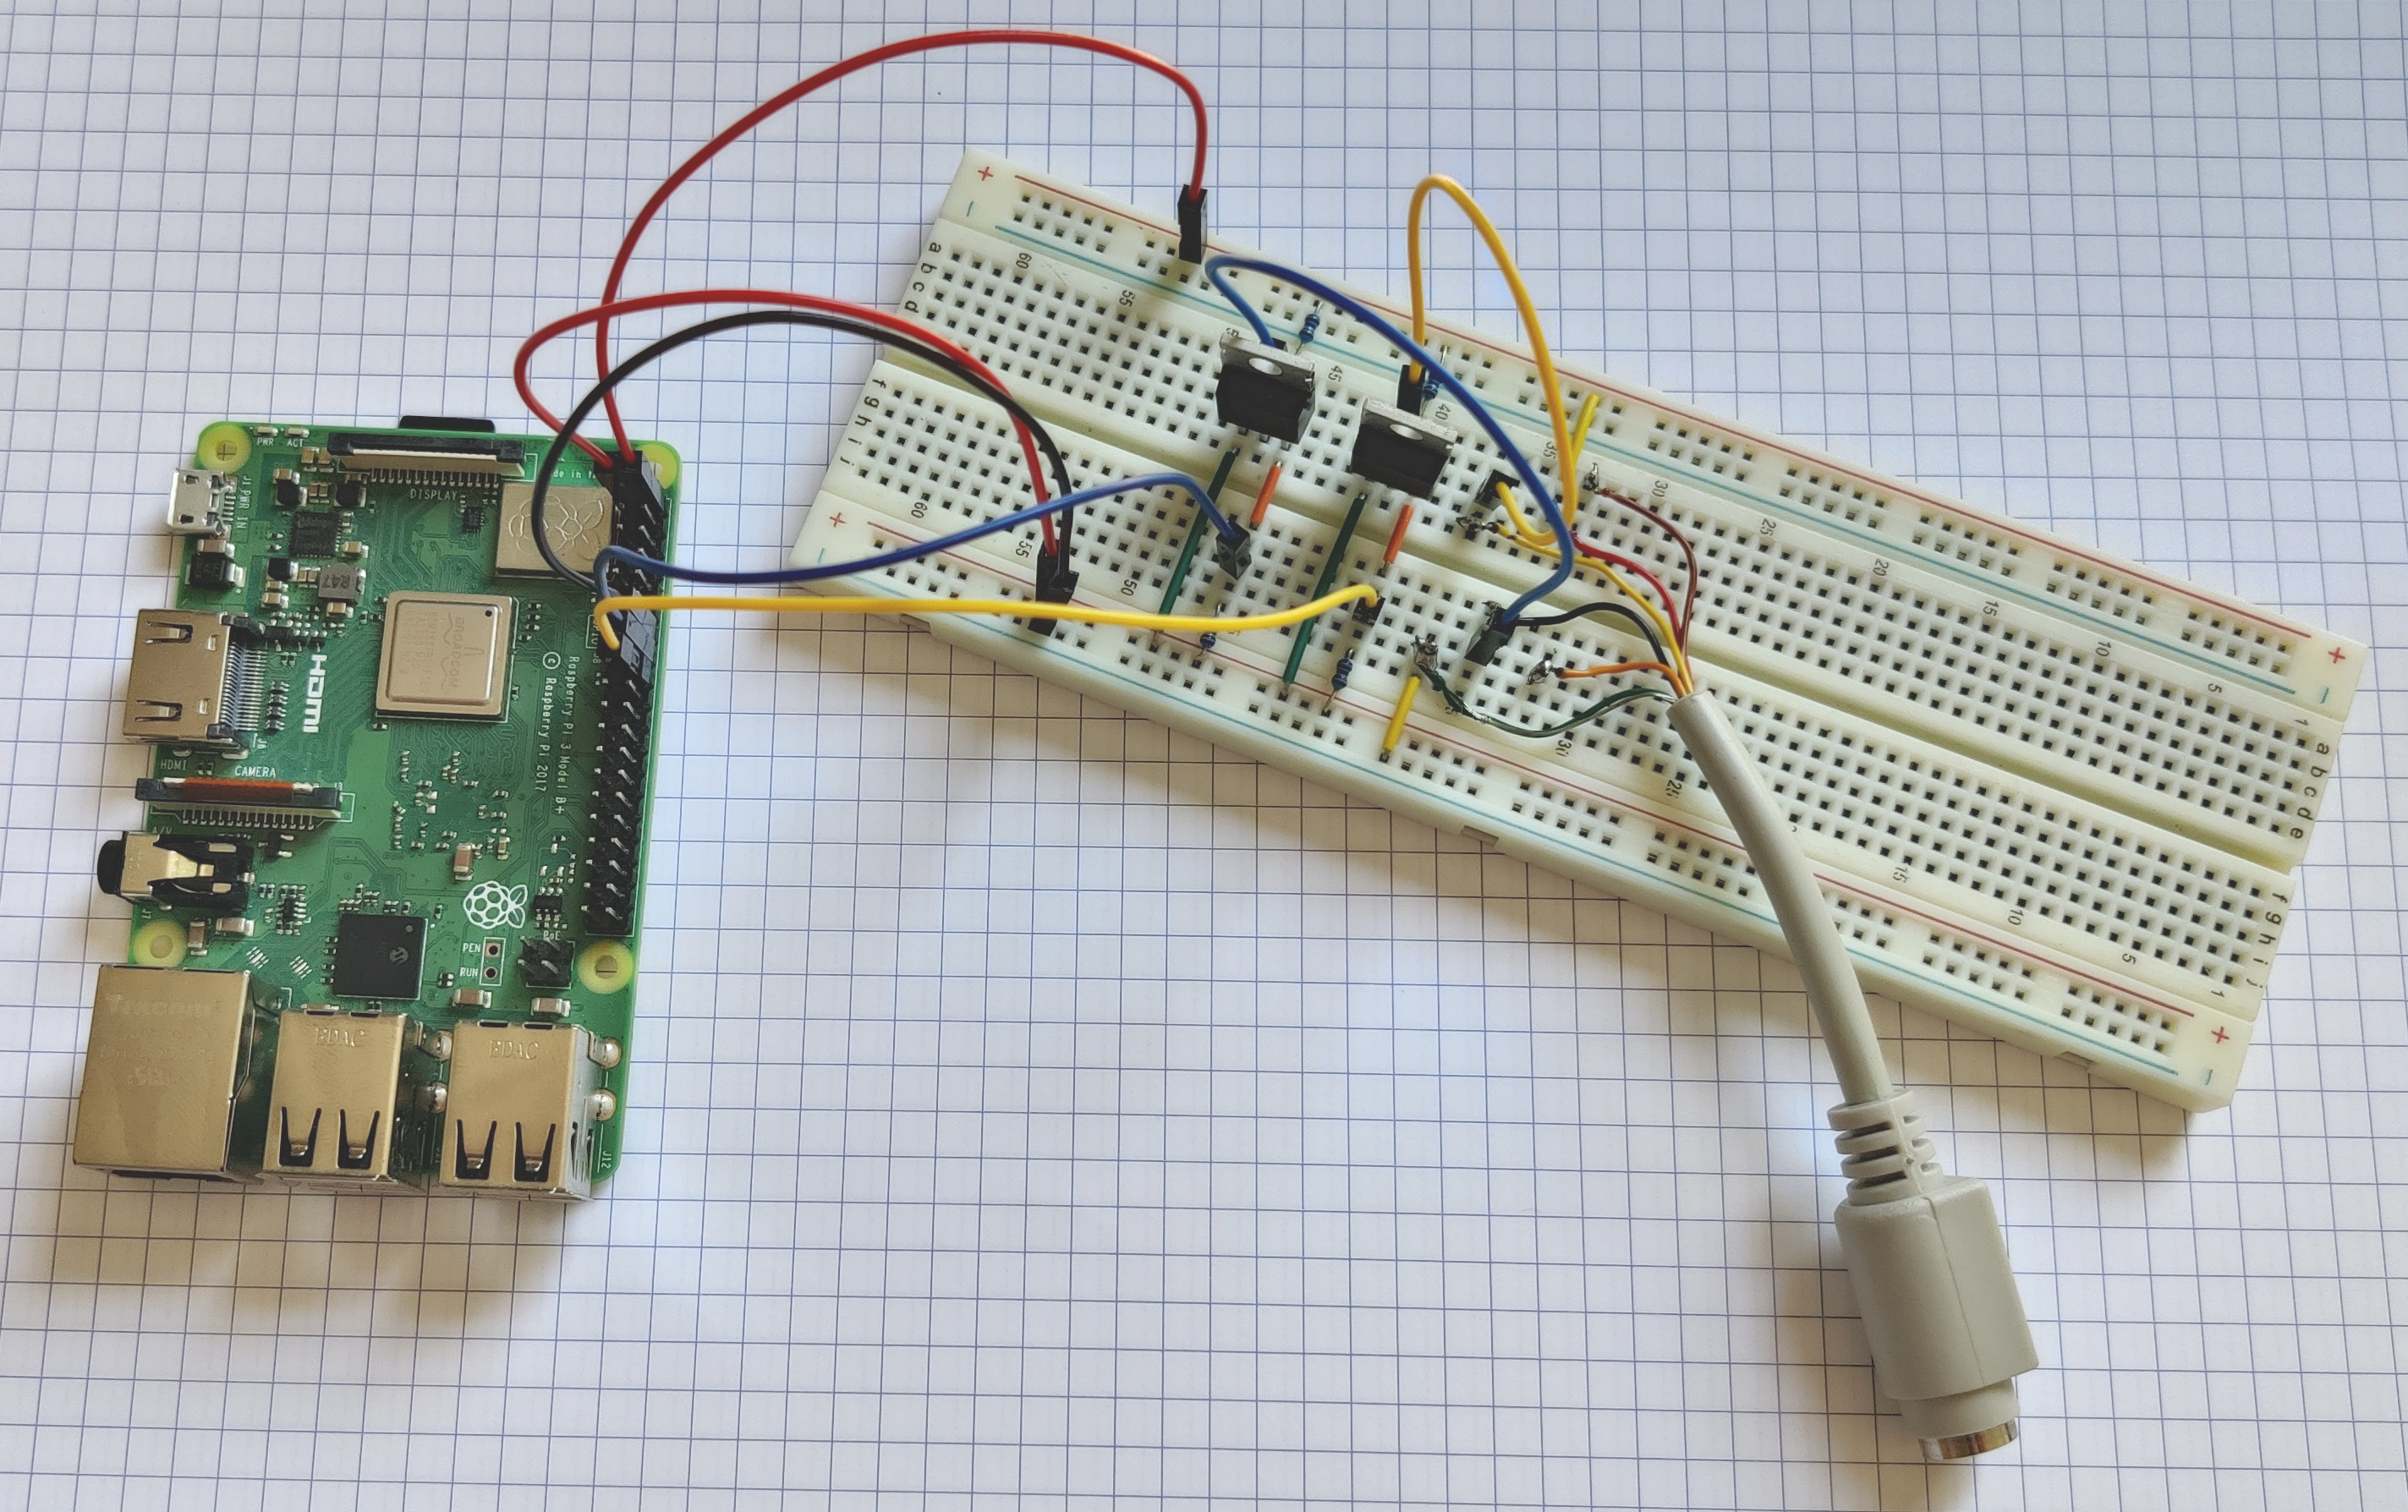
\includegraphics[height=7cm]{ps2-cables.jpg}
    \end{center}
    \caption{Le circuit électronique utilisé pour interfacer un clavier PS/2
        avec une \rpi{}.}
    \label{img:ps2-cables}
\end{figure}

Ce circuit d'alimenter et d'abaisser la tension de sortie des clavier PS/2 de
$\SI{5}{\volt}$ au $\SI{3.3}{\volt}$ supportés par le \textit{GPIO} des \rpi{}.
Le pilote PS/2, visible dans le fichier \texttt{ps2\_keyboard.cpp} est fait pour
qu'à chaque front descendant de l'horloge (en bleu sur le circuit de la figure
\ref{img:ps2-cables}), une interruption est générée et permet de lire un
bit d'information sur le fil pour les données (en jaune sur le circuit).

Après réception des 11 bits constituant un message du protocole PS/2, ce pilote
s'occupe de traiter ce message afin d'en générer des événements claviers
classiques. Ces derniers sont ensuite dispatché au \textit{handler} configuré au
sein du noyau.

\end{document}
